\documentclass{beamer}

\graphicspath{ {Paper/images/} }
\usepackage[]{inputenc, textcomp,environ,
%,geometry,graphicx,color,setspace,sectsty,comment,footmisc,
%natbib,pdflscape,subfigure,array,hyperref, booktabs,
threeparttable, siunitx, adjustbox
}

%% Resize figures and tables
% https://www.patrickbaylis.com/posts/2018-10-11-beamer-resizing/

%
% Custom font for a frame.
% 3 arguments: the size for the different itemize level
% Latex size:
% https://www.sascha-frank.com/latex-font-size.html
\newcommand{\customframefont}[3]{
    \setbeamertemplate{itemize/enumerate body begin}{#1}
    \setbeamertemplate{itemize/enumerate subbody begin}{#2}
    \setbeamertemplate{itemize/enumerate subsubbody begin}{#3}
}

%%% Create function to reduce size frame
\NewEnviron{framefont}[3]{
    \customframefont{#1}{#2}{#3} % for itemize/enumerate
    {#1 % For the text outside itemize/enumerate
        \BODY
    }
    %\customframefont{\normalsize}
}



\title[Paper banks and environment] %optional
{Financial Dependencies, Environmental Regulation, and Pollution Intensity: Evidence From China}

\author[] % (optional, for multiple authors)
{Mathilde Maurel\inst{1, 2} \and Thomas Pernet\inst{1} \and Zhao Ruili\inst{3}}
 
\institute[] % (optional)
{
  \inst{1}%
  CNRS, France
  \and
  \inst{2}%
  Centre d'Economie de la Sorbonne, Université Paris 1 Panthéon-Sorbonne, France
  \and
  \inst{3}%
  Shanghai University of International Business and Economics, China
}
 
\date[] % (optional)
{SIDE-ISLE, 19-21 December 2019}

\begin{document}

\frame{\titlepage}

\begin{frame}

\frametitle{Table of Contents}
\tableofcontents
\end{frame}

\section{Introduction}

\begin{framefont}{\small}{\footnotesize}{\footnotesize}
    \begin{frame}{The environment's emergency}
        \begin{itemize}
            \item{A need to switch toward a cleaner model of economic growth}
                \begin{itemize}
                    \item{Particularly in fast growing middle-class economies (China, India)}
                \end{itemize}
            \item{Environmental issues in China is growing dramatically}
                \begin{itemize}
                    \item{Largest COD emitters in the world in 2006}
                    \item{Hosts more than half of the most polluted cities in the world}
                    \item{An average province in China has a direct loss due to natural disasters of about \$3B}
                    \begin{figure}[ht]
                        \centering
                        \textbf{}\par\medskip
                        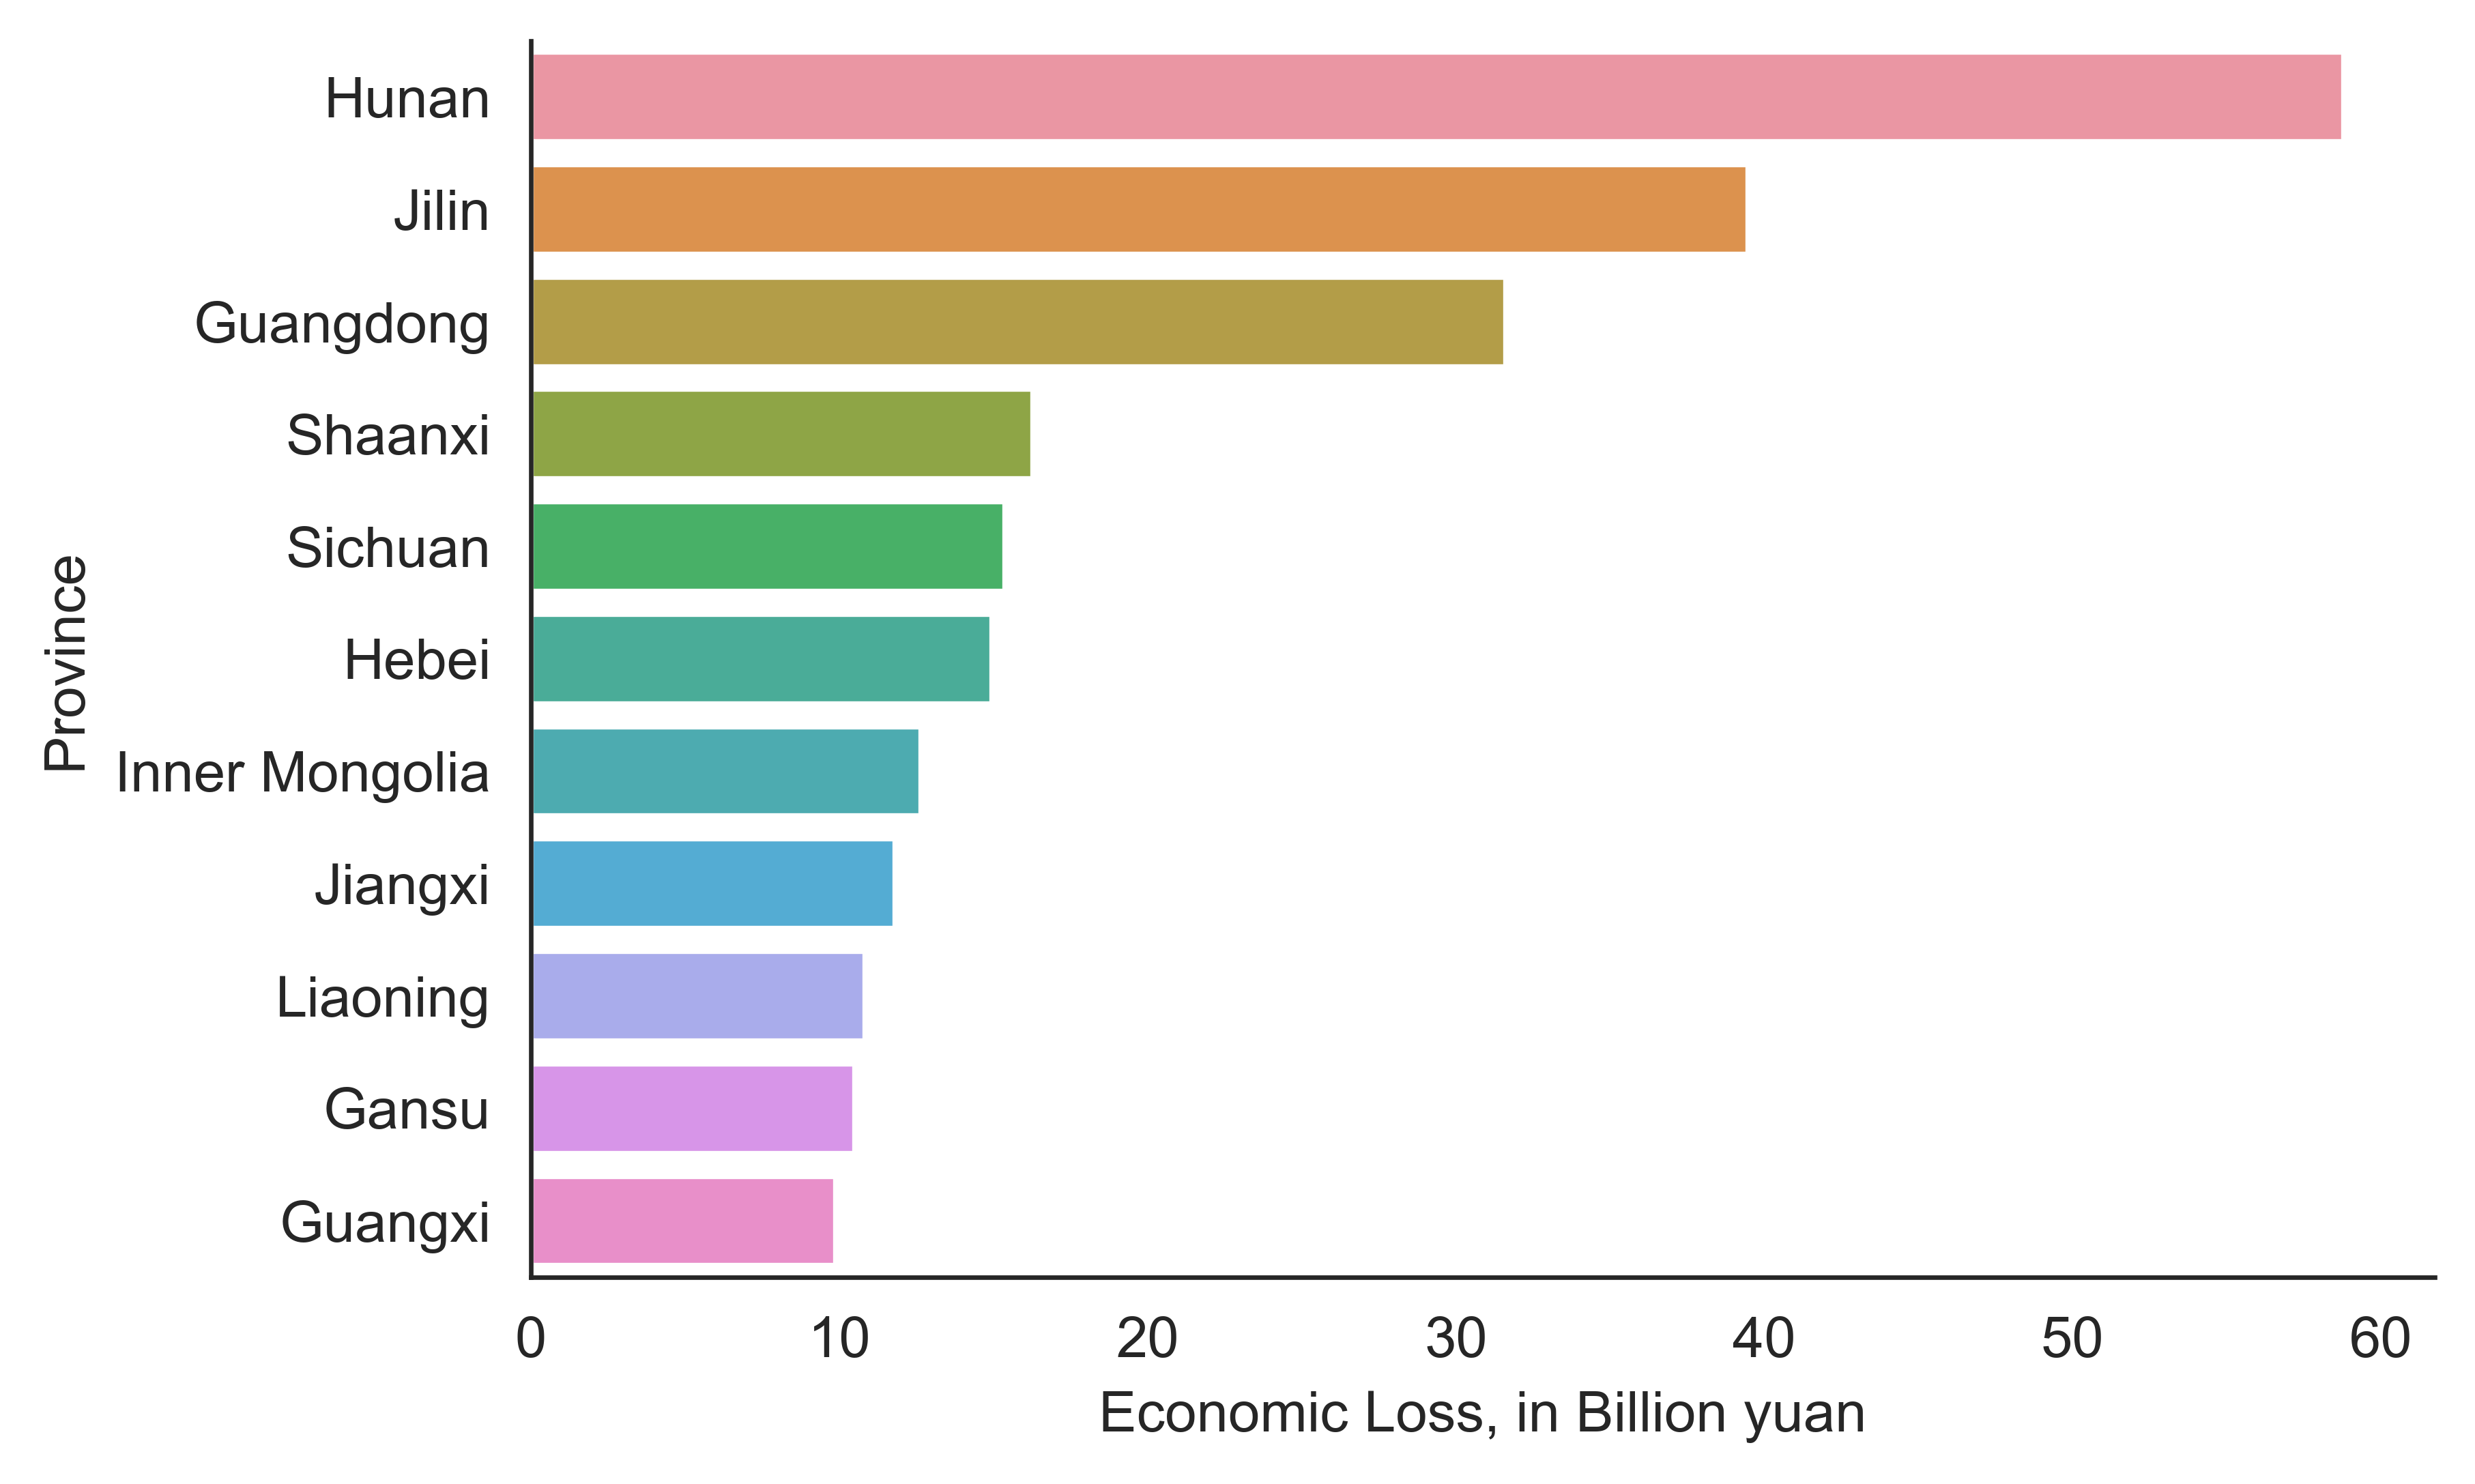
\includegraphics[width=0.6\textwidth]{Econ_loss_presentation.png}\\
                       \scriptsize \textbf{Source}: National Bureau of Statistics of China; Ministry of Ecology and Environment (China)
                    \end{figure}
            \end{itemize}
        \end{itemize}
    \end{frame}
\end{framefont}

\begin{frame}{Related Researches}

\centering How to improve environmental's metrics?
    \begin{itemize}
        \item{Previous researches}
        \begin{itemize}
            \item Literature emphasises on the reallocation of production away from polluting sectors 
            \item Little research paid attention to the relationship between the financial system and environmental issues
        \end{itemize}
        \item Our research
        \begin{itemize}
            \item How banks' involvement in a firm’s financing may be in line with environmental policies pursued by the central government
        \end{itemize}
    \end{itemize}
\end{frame}

\begin{framefont}{\small}{\scriptsize}{\scriptsize}
    \begin{frame}{The choice of China}
    \begin{itemize}
        \item China is a perfect candidate for three reasons
            \begin{itemize}
                \item  The Chinese financial market went through rapid reform over a short time span to cope with the transition to a market-driven economy
                \item Launch of exhaustive environmental policy: a set of quantitative measures of pollution reduction targets at the national and local levels, spread unequally across provinces, with some provinces being required to exert higher efforts and some others lower efforts
                \item A rich dataset about major pollutants such as sulfur dioxide, wastewater, chemical oxygen demand as well as industrial dust covering all the industrial sectors through time
            \end{itemize}
         \item Our idea to bring together these three points and link it to the decrease of SO2 after 2006 with a DDD
        \begin{figure}[ht]
            \centering
            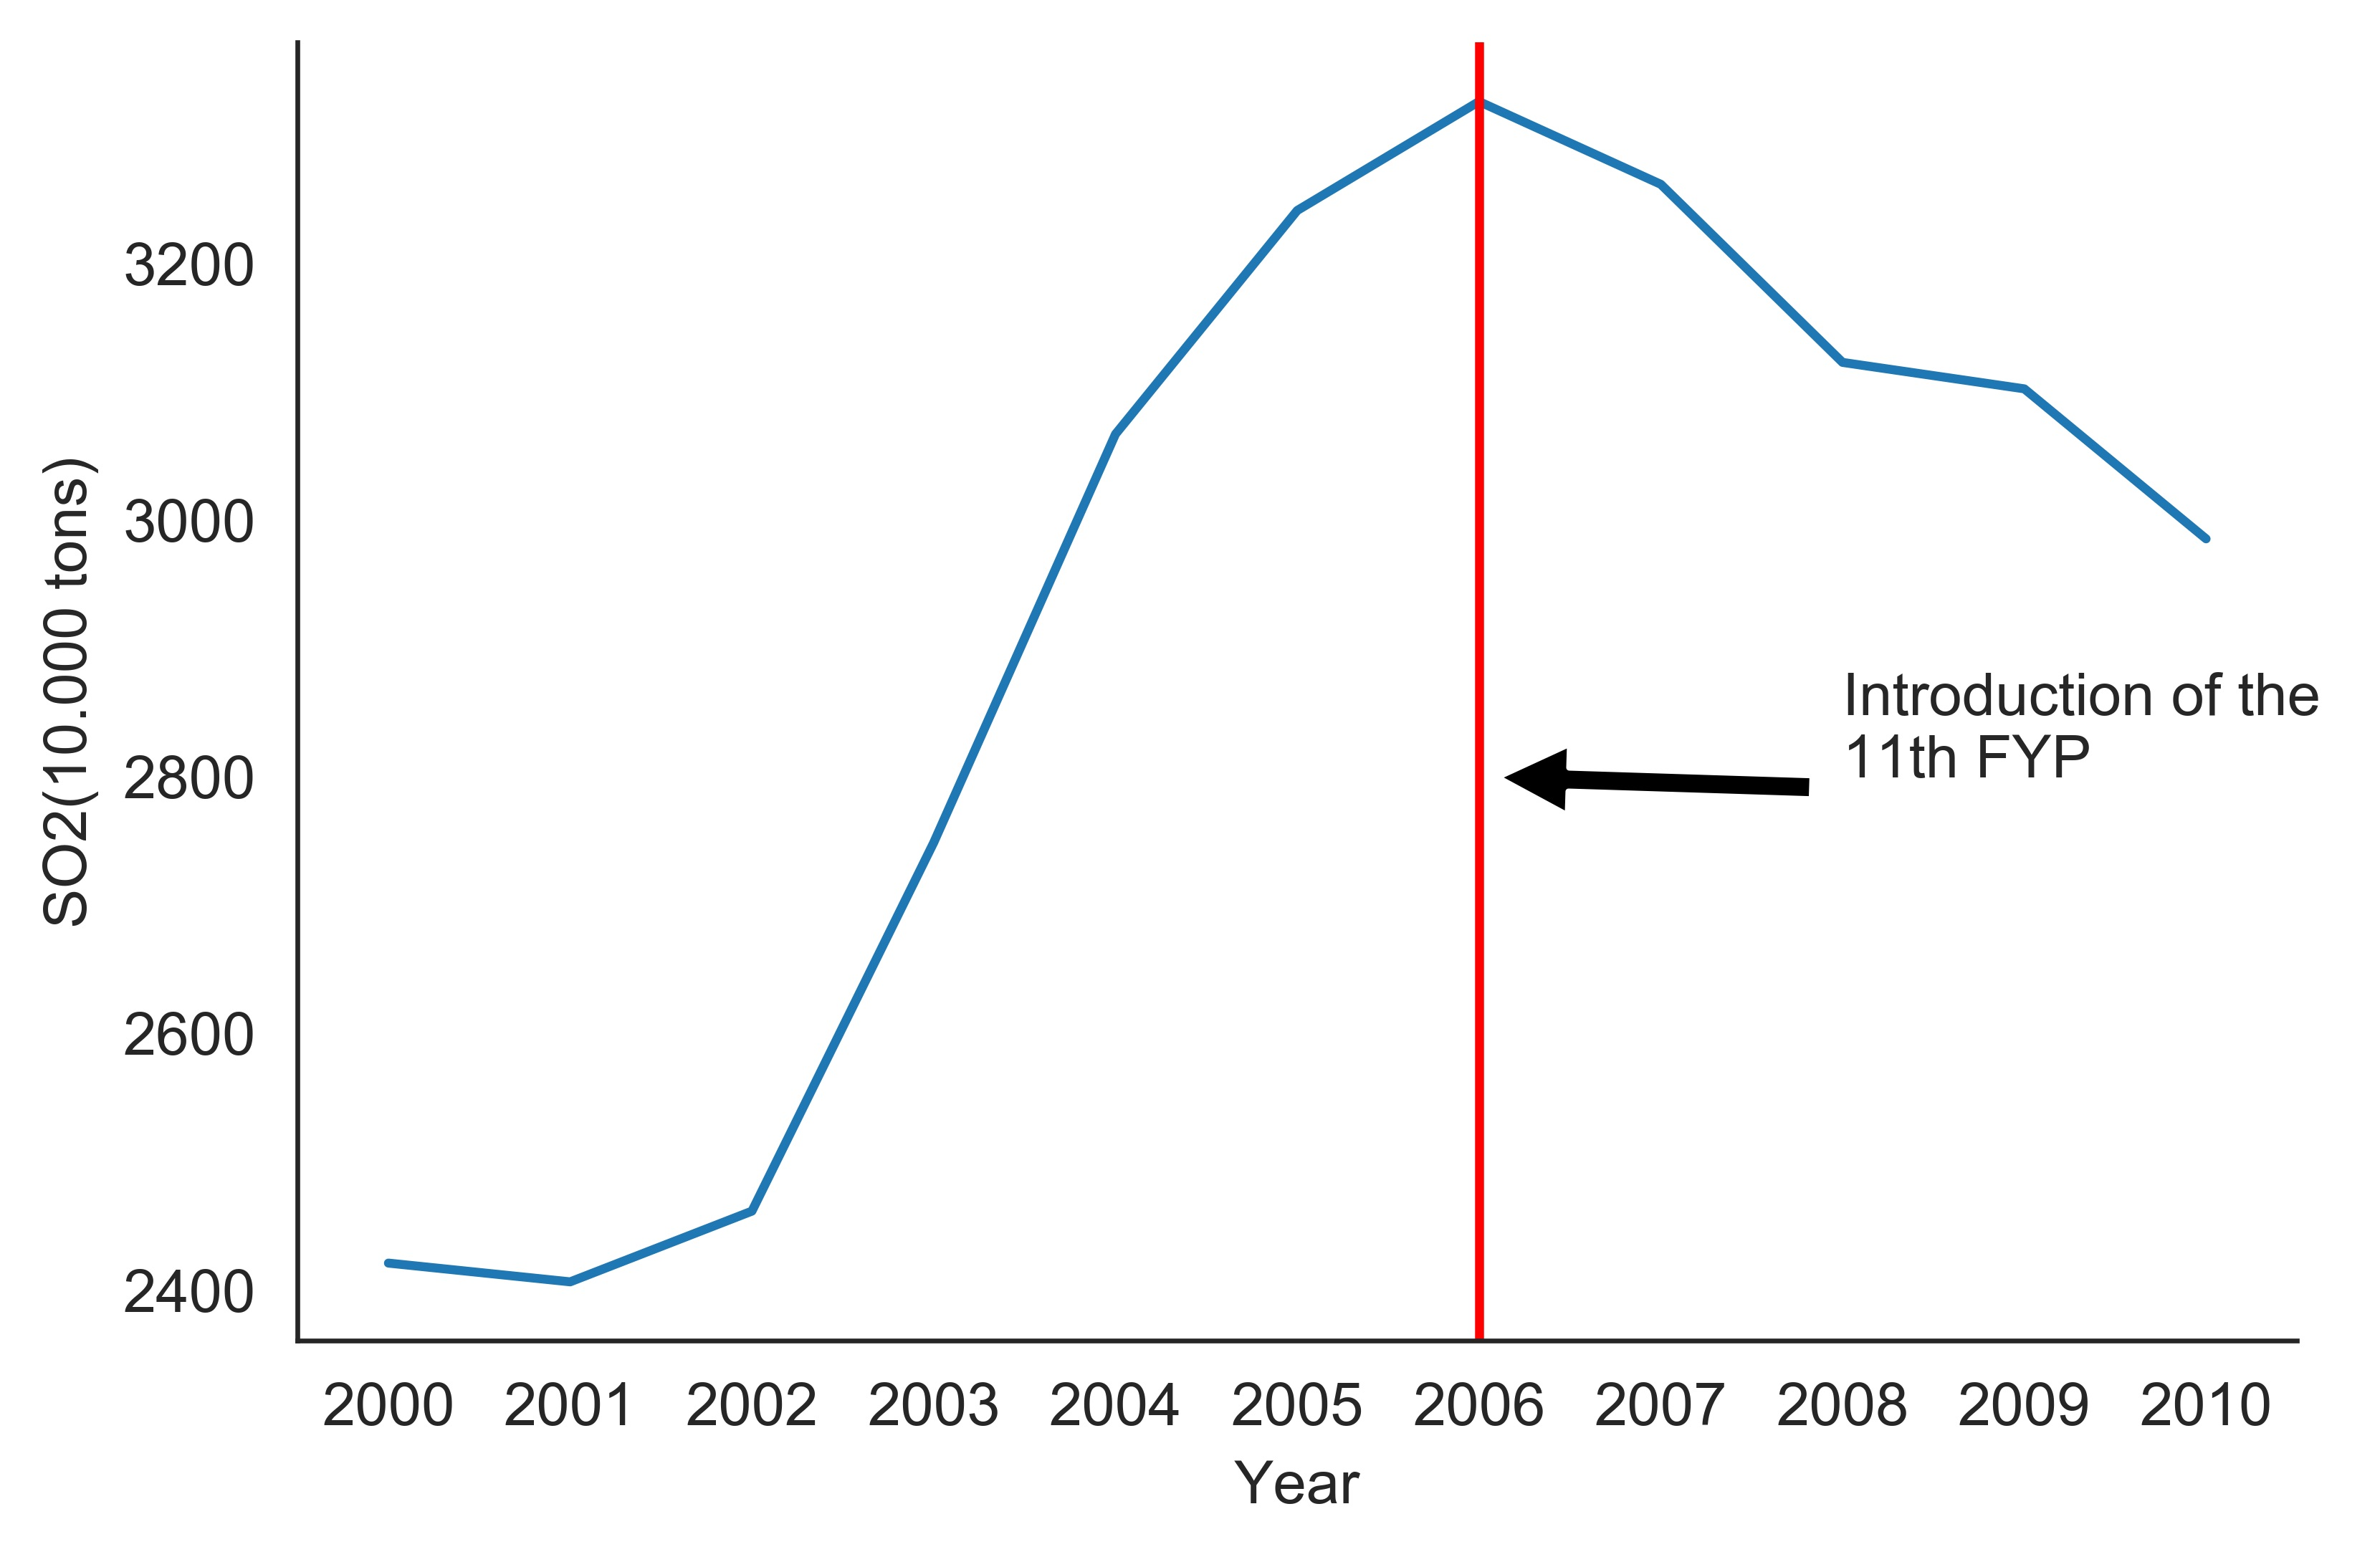
\includegraphics[width=0.5\textwidth]{fig_1}\\
            \tiny \textbf{Source}: The SO2 emission data are from the \href{http://www.stats.gov.cn/english/Statisticaldata/AnnualData/}{China Statistical Yearbook (2000, 2010)}
        \end{figure}
    \end{itemize}
    \end{frame}
\end{framefont}

\begin{frame}{Results}
    \begin{itemize}
        \item Estimate the effect of the credit reallocation induced by the shift of policy emphasis towards environmental concerns after 2006 on the emission of SO2
        \begin{enumerate}
            \item Strong evidence that there is a connection between the allocation of credit and the environmental policies: Banks favour sustainable finance only when they are constrained by the lawmakers
            \begin{itemize}
                \item   average city can save up to 62 million USD per year of environmental damage by moving on tougher environmental objective
            \end{itemize}
             \item A stronger deterrent effect of environmental regulation leads firms to seek funding in less restricted provinces, confirming the pollution haven hypothesis (PVH)
        \end{enumerate}
    \end{itemize}
\end{frame}

\section{Environmental policy in China}

\begin{frame}{Environmental policy in China: 10th FYP}
    \begin{itemize}
        \item  From a national environmental policy ...
        \begin{itemize}
            \item   10th FYP (2001-2005) adds a 10\% SO2 national reduction objective \textrightarrow Large failure
            \begin{enumerate}
                \item Banks have always provided credits to large industrial firms in order to promote industrialisation
                \item State Environmental Protection Administration (SEPA) turns out to be a weak regulatory agency
                \item Local governments were not under threat of sanctions if they failed
            \end{enumerate}
        \end{itemize}
    \end{itemize}
\end{frame}

\begin{frame}{Environmental policy in China: 11th FYP}
    \begin{itemize}
        \item ...to a local objective
            \begin{itemize}
                \item   During the 11th FYP (2006-2009), enforces the 10\% mandate with more constraints at the local level
            \begin{enumerate}
                \item local leaders’ career opportunities are made dependent on the achievement of environmental objectives
                \item The market-based policy instruments in favor of pollution reduction and environmental protection came in addition to the existing environmental laws and regulations
                \item  An improvement of the communication between SEPA and commercial banks allowed to limit or even reject loans to firms infringing environmental laws
                \item By the end of 2009, the total amount of investment geared toward the environment reached 1.33\% of the GDP, a yearly increase of 15\% since 2005
            \end{enumerate}
        \end{itemize}
    \end{itemize}
\end{frame}

\section{Estimation strategy and Variables}

\begin{framefont}{\small}{\scriptsize}{\scriptsize}
    \begin{frame}{Empirical strategy}
        \begin{itemize}
            \item Assess the effect of credit reallocation on the emission of pollution when banks face stringent environmental policies
            \begin{itemize}
                \item Banks allocate resources to firms that comply with environmental regulations and with the objectives of reducing pollution
            \end{itemize}
            \item DDD: Policy and Time and Financial dependency
            \begin{enumerate}
                \item  Policy & Time
                \begin{itemize}
                    \item lawmakers assigned in 2006 to cities different levels of SO2 to be met within the time span of the FYP: the existence of a treatment year (before and after 2006)
                \end{itemize}
                \item  Role of banks proxied by Financial dependency
                \begin{itemize}
                    \item firms dependent on banks are more likely to react to the new regulation when banks confronted with the new regulation can reallocate the credit away from polluting projects
                \end{itemize}
                \item The advantage of the triple differences is the possibility to include a full of city-industry, city-year, and industry-year fixed effects
            \end{enumerate}
            \begin{equation*}
                SO2_{ckt} = \alpha\text{Financial Dependencies}_{k} \times Post_{t} \times \text{Reduction Mandate}_{c} + \\
                \beta X_{ckt} + \mu_{ct} + \gamma{kt} + \delta{ck} + \epsilon_{ckt}
            \end{equation*}
        \end{itemize}
    \end{frame}
\end{framefont}

\begin{framefont}{\small}{\scriptsize}{\scriptsize}
    \begin{frame}{Variables}
        \begin{itemize}
            \item SO2
            \begin{itemize}
                \item The Ministry of Environment (MEP) collects the main data source about pollutants and wastes in China since 1980
                \item The MEP implemented strict procedures, including unforeseen visits from experts to ensure that firms did not misreport their emissions
                \item SO2 statistics, a primary air pollutant, for 28 two digits industry, spread across 289 cities from 2002 to 2007
            \end{itemize}
            \item City reduction
            \begin{itemize}
                \item  City reduction mandate is not directly observable, we estimate it as follow:
            
                \tiny \begin{equation*}
                    \Delta SO2_{c, 05 - 10}=\Delta SO2_{p, 05 - 10} \times \sum_{k=1}^{29} \mu_{k} \frac{\text { output value of industry } k \text { in city } c}{\text { output value of industry } k \text { in province } p}
                \end{equation*}
                \item Shanghai is intended to reduce its SO2 emissions by 13.000 tons in 2010
            \end{itemize}
            \item Financial dependencies: sector-level reliance on external finance
            \begin{itemize}
                \item Use the industry’s external finance dependency defined as the exposure of industry to the banks
                \item It is the share of capital expenditure not financed with cash flow from operations
                \begin{enumerate}
                    \item Use the Chinese date and replicate the methodology proposed by Fan, Lai, and Li (2015)
                    \item Use the ASIF dataset during the years 2004-2006 to aggregate the capital expenditure and cash flow at the two digits industrial level
                \end{enumerate}
            \end{itemize}
        \end{itemize}
    \end{frame}
\end{framefont}

\begin{framefont}{\small}{\scriptsize}{\scriptsize}
    \begin{frame}{Structure of Chinese SO2 industries}
        \begin{itemize}
            \item Objective is to disentangle the different levels of pollution when a sector faces different borrowing constraints
            \begin{enumerate}
                \item Analyses the variations of SO2 emission between the two periods by financially constrained sectors of two cities with different environmental mandates
                \begin{itemize}
                    \item The city of Tangshan belongs to the top decile of environmental severity. The city of Xiamen is on the third decile. 
                    \item Both cities share similar characteristics for GDP
                \end{itemize}
                \begin{figure}[ht]
                    \centering
                    \textbf{Financial dependencies and two economically identical cities with different environmental regulations}\par\medskip
                    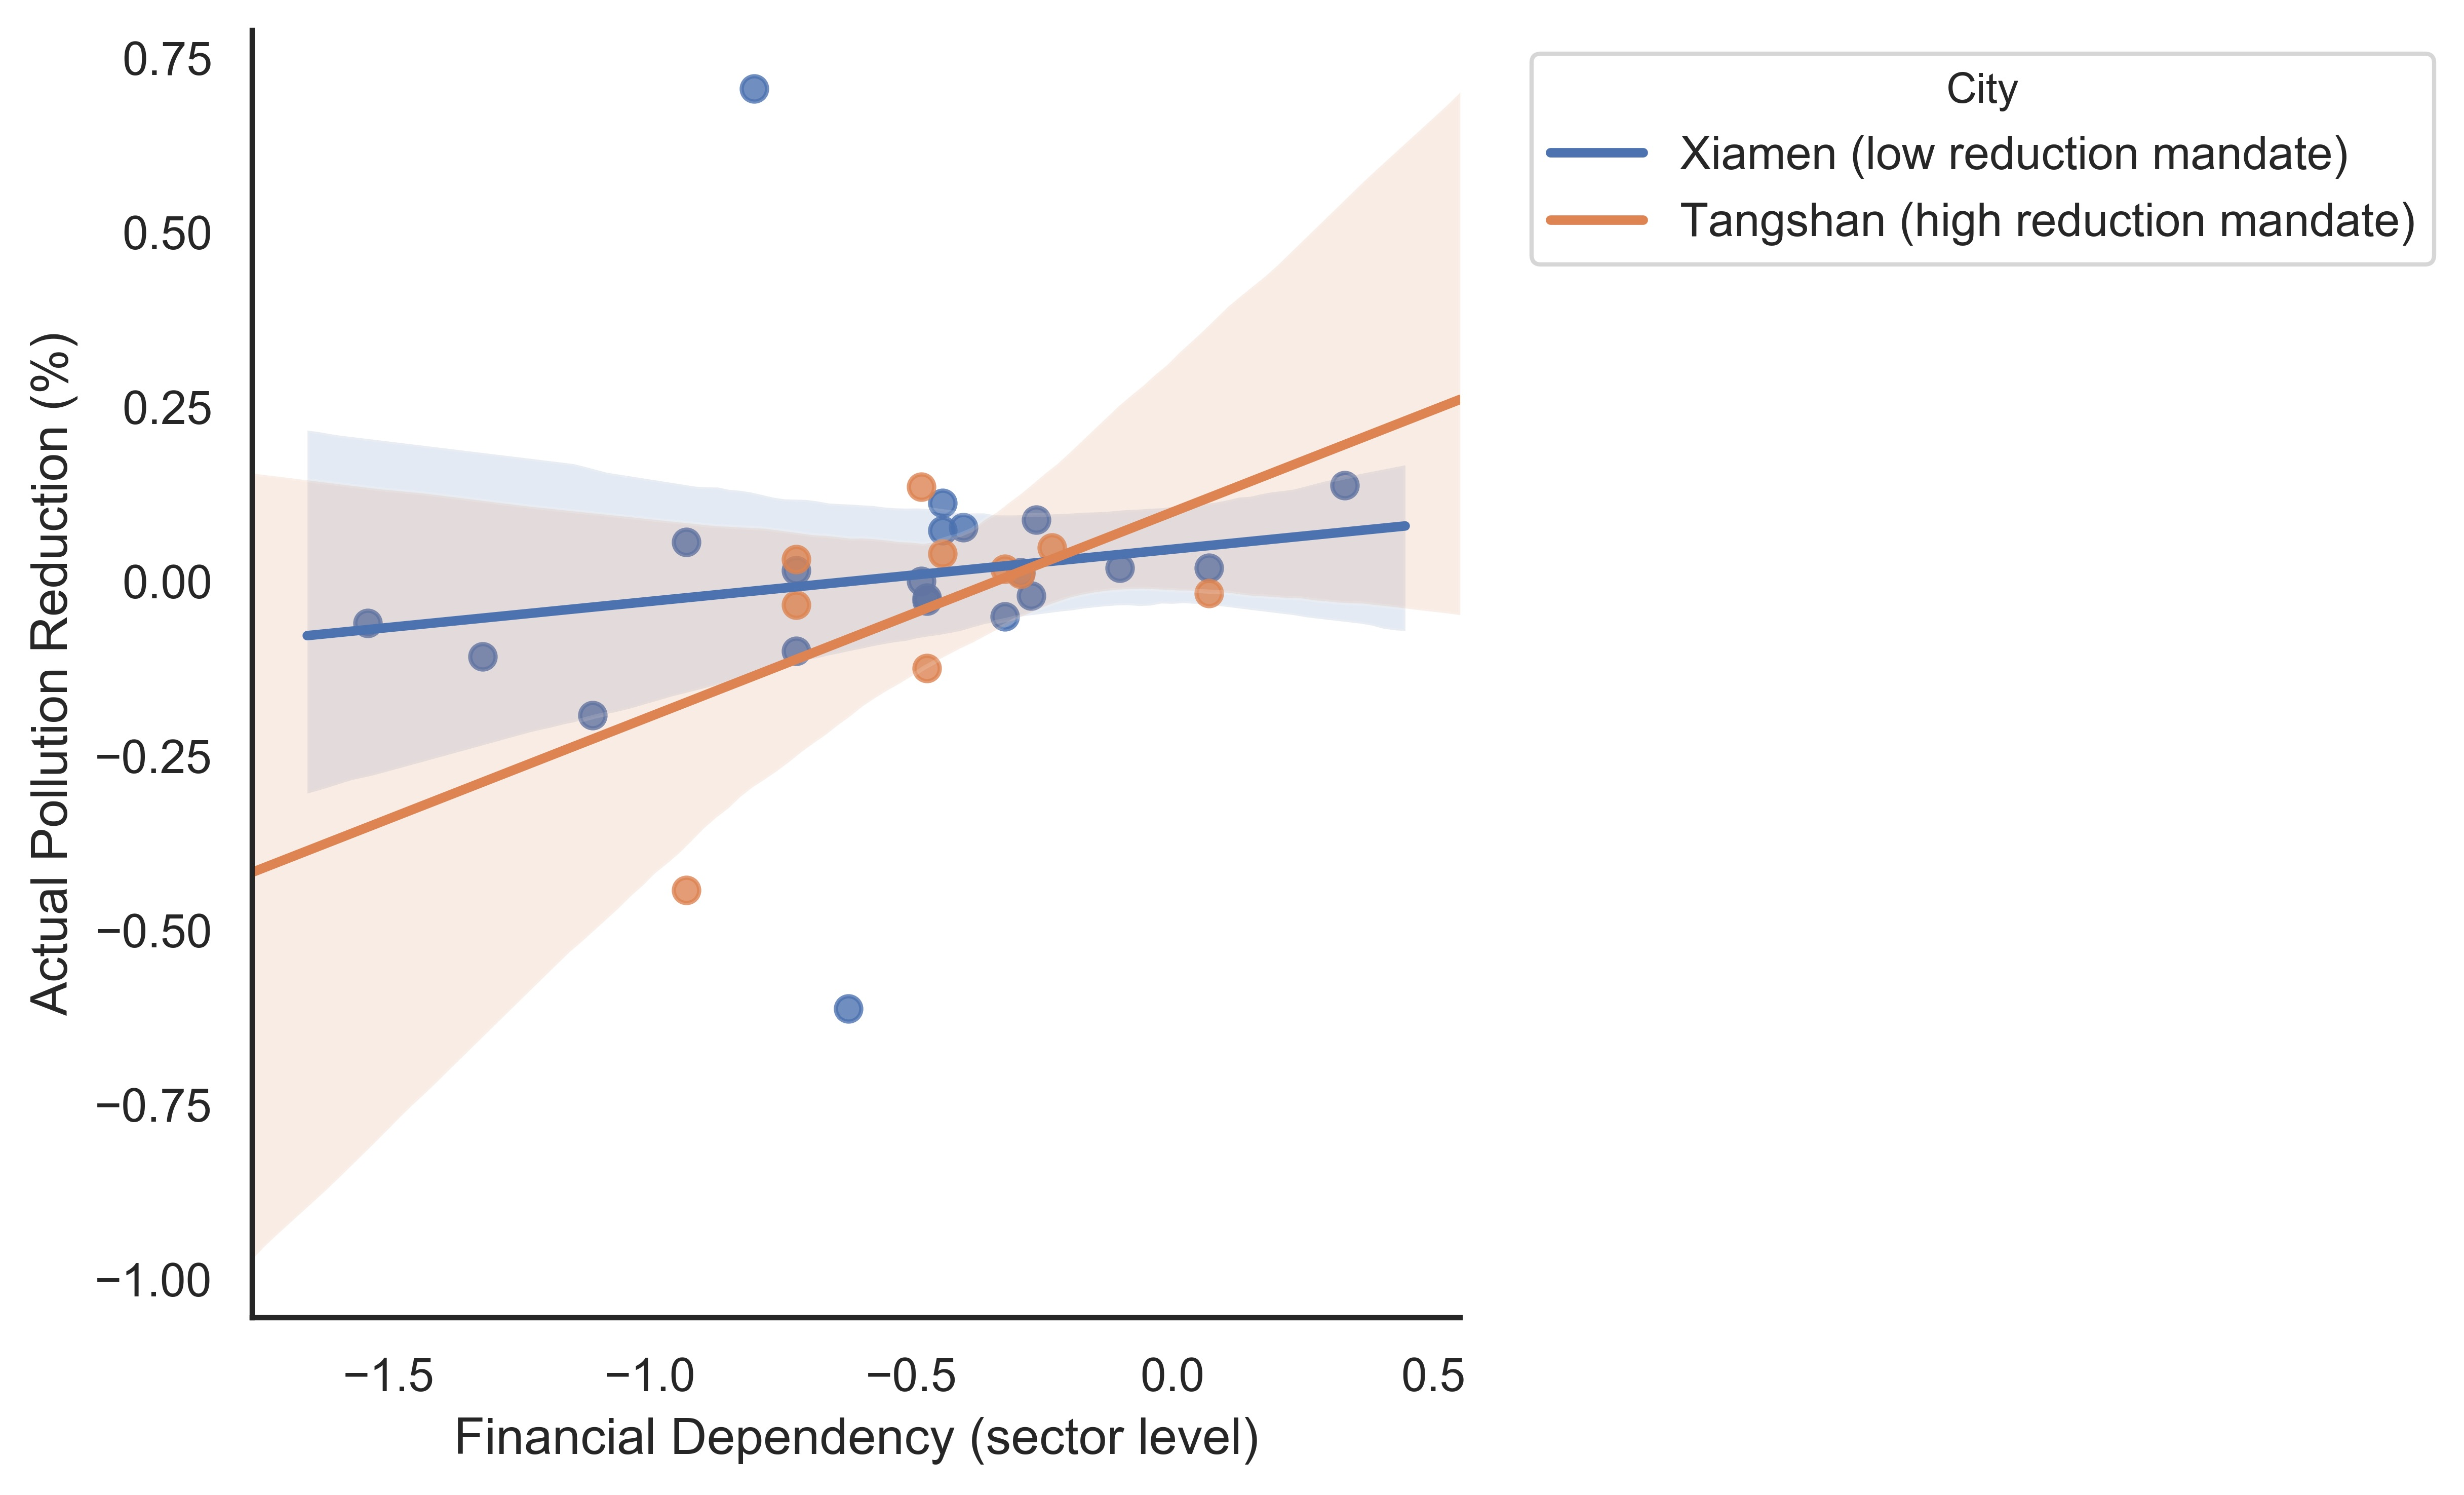
\includegraphics[width=0.7\textwidth]{fig_4}
                \end{figure}
            \end{enumerate}
        \end{itemize}
\end{frame}
\end{framefont}

\section{Results}

\begin{frame}{Main results}

    \begin{table}[htbp]\centering
        %\resizebox{1\textwidth}{!}{
        \begin{adjustbox}{width=\textwidth,
        totalheight=\textheight-2\baselineskip,keepaspectratio}
        \begin{threeparttable}   
        \caption{\small The effect of environmental regulation and financial dependency on the emission of SO2, baseline regression}
        \begin{tabular}{l*{4}{c}}
            \toprule
     
            &\multicolumn{4}{c}{} \\ 
            \hline
            & \multicolumn{2}{c}{Ln SO2} & \multicolumn{2}{c}{Ln SO2 intensity} \\
            \\[-1.8ex] & (1) & (2) & (3) & (4)\\ 
            \hline 
            $\text{Financial dep.}_k$ x Post x $\text{SO2 mandate}_c$ & $-$0.354$^{*}$ & $-$0.514$^{**}$ & $-$0.415$^{*}$ & $-$0.601$^{***}$ \\ 
            & (0.208) & (0.200) & (0.213) & (0.207)  \\
            \midrule
            Controls variables & Yes & Yes & Yes & Yes \\ 
            City-year fixed effects & Yes & Yes & Yes & Yes \\ 
            Industry-year fixed effects & Yes & Yes & Yes & Yes \\ 
            City-industry fixed effects & Yes & Yes & Yes & Yes \\ 
            Observations & 25,404 & 18,509 & 25,404 & 18,509 \\ 
            R$^{2}$ & 0.889 & 0.866 & 0.869 & 0.860 \\  
            \bottomrule
        \end{tabular}
        \begin{tablenotes}
        \scriptsize
            \item SO2 intensity is computed as the total SO2 emission by city-industry-year divided by value added. SO2 city mandate measures the total amount of SO2 a city needs to reduce by the end of the 11th FYP. Columns 2 and 4 exclude the top and bottom 4 most polluted sectors in 2002.All columns controls for the output, fixed asset and employment computed at the city, industry, year. \\
            * Significance at the 10\%, ** Significance at the 5\%, *** Significance at the 1\%. Heteroskedasticity-robust standard errors in parentheses are two-way clustered by city and by industry.
        \end{tablenotes}
        \end{threeparttable}
        \end{adjustbox}
        %}
    \end{table}
\end{frame}

\begin{frame}{Parallel trend}

    \begin{table}[htbp]\centering
        %\resizebox{1\textwidth}{!}{
        \begin{adjustbox}{width=\textwidth,
        totalheight=\textheight-2\baselineskip,keepaspectratio}
        \begin{threeparttable}   
            \caption{\small The effect of environmental regulation and financial dependency on the emission of SO2, testing the parallel trend assumption}
            \begin{tabular}{l*{2}{c}}
    %\multicolumn{1}{l}{\textbf{\small The effect of environmental %regulation and financial dependency on the emission of SO2, %testing the parallel trend assumption}} \\
                \toprule
                & \multicolumn{2}{c}{} \\ 
                \hline
             & \multicolumn{1}{c}{Ln SO2} & \multicolumn{1}{c}{Ln SO2 intensity} \\ 
                \\[-1.8ex] & (1) & (2) \\ 
                \hline
                $\text{Financial dep.}_k$ x Year 2003 x $\text{SO2 mandate}_c$ & $-$0.236 & $-$0.240 \\ 
                & (0.225) & (0.235) \\ 
                $\text{Financial dep.}_k$ x Year 2004 x $\text{SO2 mandate}_c$ & $-$0.276 & $-$0.288 \\ 
                & (0.257) & (0.256) \\ 
                $\text{Financial dep.}_k$ x Year 2005 x $\text{SO2 mandate}_c$ & $-$0.383 & $-$0.445 \\ 
                & (0.242) & (0.282) \\ 
                $\text{Financial dep.}_k$ x Year 2006 x $\text{SO2 mandate}_c$ & $-$0.567$^{*}$ & $-$0.641$^{*}$ \\ 
                & (0.344) & (0.333) \\ 
                $\text{Financial dep.}_k$ x Year 2007 x $\text{SO2 mandate}_c$ & $-$0.594$^{**}$ & $-$0.682$^{**}$ \\ 
                & (0.290) & (0.329) \\  
                \midrule
                City-year fixed effects & Yes & Yes  \\ 
                Industry-year fixed effects & Yes & Yes  \\ 
                City-industry fixed effects & Yes & Yes  \\ 
                Observations & 25,404 & 25,404 \\ 
                R$^{2}$ & 0.889 & 0.869 \\  
                \bottomrule
            \end{tabular}
            \begin{tablenotes}
                \scriptsize
                \item The year 2002 is the omitted category. SO2 intensity is computed as the total SO2 emission by city-industry-year divided by value added. All columns controls for the output, fixed asset and employment computed at the city, industry, year. \\
                * Significance at the 10\%, ** Significance at the 5\%, *** Significance at the 1\%. Heteroskedasticity-robust standard errors in parentheses are two-way clustered by city and by industry.
            \end{tablenotes}
        \end{threeparttable}
        \end{adjustbox}
        %}
    \end{table}
\end{frame}

\begin{frame}{Heterogeneous effects}
    \begin{itemize}
        \item Test average SO2 reduction effect differs according to firms’ ownership and firms’ size
        \begin{enumerate}
            \item SOE vs Private
            \begin{itemize}
                \item  Test credit allocation is biased in favor of state-owned enterprises
                \item  China's political pecking order of firms is enforced through the systematic misallocation of financial resources
            \end{itemize}
            \item Domestic vs Foreign
            \begin{itemize}
                \item  Test credit allocation is irrelevant for Foreign firms and significant for Domestic
                \item Foreign firms can get funding from the parents' company to raise money on the capital market
            \end{itemize}
            \item Large vs Small
            \begin{itemize}
                \item Test credit allocation favored for Large firms
                \item Large companies have easier access to external financing
                \item Large firms have more collateral to pledge
            \end{itemize}
        \end{enumerate}
    \end{itemize}
    
\end{frame}

\begin{frame}{Reallocation effect}

    \begin{itemize}
        \item Test the Polution Haven Hypothesis
        \begin{itemize}
            \item Investigate whether firms seek to circumvent the environmental regulation by relocating in cities with less environmental concerns and moving away part of their polluting activities from the more regulated cities
            \item Firms’ owners can decide to reduce the production in cities with strict environmental policy and invests in factories located in areas with less environmental requirements
            \item The decrease in pollution results of a haven effect, more polluting firms being pushed away from more demanding cities in terms of S02 emission
        \end{itemize}
    \end{itemize}
\end{frame}

\section{Conclusion}

\begin{frame}{Take Away}
    \begin{itemize}
        \item Spatial and temporal variations of environmental policy enacted by the 11th Five-Year Plan allow us to isolate the impact of financial dependency on the emission of air pollution
        \item We find evidence that stricter environmental policy leads to a deeper decline in emissions of SO2 in industries dependent on external borrowing
        \begin{enumerate}
            \item banks have more incentives to provide funding to firms that comply with the environmental objectives announced by the government
            \item  The effect of credit reallocation has more significant impacts on industries dominated by private, domestic, and large firms
        \end{enumerate}
        \item The spatial disparity of the regulation leads firms operating in stringent areas to look for funding in cities where banks are less preoccupied with the use of capital on the environment
    \end{itemize}
    
\end{frame}

\end{document}